% Options for packages loaded elsewhere
\PassOptionsToPackage{unicode}{hyperref}
\PassOptionsToPackage{hyphens}{url}
\PassOptionsToPackage{dvipsnames,svgnames,x11names}{xcolor}
%
\documentclass[
  letterpaper,
  DIV=11,
  numbers=noendperiod]{scrartcl}

\usepackage{amsmath,amssymb}
\usepackage{iftex}
\ifPDFTeX
  \usepackage[T1]{fontenc}
  \usepackage[utf8]{inputenc}
  \usepackage{textcomp} % provide euro and other symbols
\else % if luatex or xetex
  \usepackage{unicode-math}
  \defaultfontfeatures{Scale=MatchLowercase}
  \defaultfontfeatures[\rmfamily]{Ligatures=TeX,Scale=1}
\fi
\usepackage{lmodern}
\ifPDFTeX\else  
    % xetex/luatex font selection
\fi
% Use upquote if available, for straight quotes in verbatim environments
\IfFileExists{upquote.sty}{\usepackage{upquote}}{}
\IfFileExists{microtype.sty}{% use microtype if available
  \usepackage[]{microtype}
  \UseMicrotypeSet[protrusion]{basicmath} % disable protrusion for tt fonts
}{}
\makeatletter
\@ifundefined{KOMAClassName}{% if non-KOMA class
  \IfFileExists{parskip.sty}{%
    \usepackage{parskip}
  }{% else
    \setlength{\parindent}{0pt}
    \setlength{\parskip}{6pt plus 2pt minus 1pt}}
}{% if KOMA class
  \KOMAoptions{parskip=half}}
\makeatother
\usepackage{xcolor}
\setlength{\emergencystretch}{3em} % prevent overfull lines
\setcounter{secnumdepth}{5}
% Make \paragraph and \subparagraph free-standing
\makeatletter
\ifx\paragraph\undefined\else
  \let\oldparagraph\paragraph
  \renewcommand{\paragraph}{
    \@ifstar
      \xxxParagraphStar
      \xxxParagraphNoStar
  }
  \newcommand{\xxxParagraphStar}[1]{\oldparagraph*{#1}\mbox{}}
  \newcommand{\xxxParagraphNoStar}[1]{\oldparagraph{#1}\mbox{}}
\fi
\ifx\subparagraph\undefined\else
  \let\oldsubparagraph\subparagraph
  \renewcommand{\subparagraph}{
    \@ifstar
      \xxxSubParagraphStar
      \xxxSubParagraphNoStar
  }
  \newcommand{\xxxSubParagraphStar}[1]{\oldsubparagraph*{#1}\mbox{}}
  \newcommand{\xxxSubParagraphNoStar}[1]{\oldsubparagraph{#1}\mbox{}}
\fi
\makeatother


\providecommand{\tightlist}{%
  \setlength{\itemsep}{0pt}\setlength{\parskip}{0pt}}\usepackage{longtable,booktabs,array}
\usepackage{calc} % for calculating minipage widths
% Correct order of tables after \paragraph or \subparagraph
\usepackage{etoolbox}
\makeatletter
\patchcmd\longtable{\par}{\if@noskipsec\mbox{}\fi\par}{}{}
\makeatother
% Allow footnotes in longtable head/foot
\IfFileExists{footnotehyper.sty}{\usepackage{footnotehyper}}{\usepackage{footnote}}
\makesavenoteenv{longtable}
\usepackage{graphicx}
\makeatletter
\newsavebox\pandoc@box
\newcommand*\pandocbounded[1]{% scales image to fit in text height/width
  \sbox\pandoc@box{#1}%
  \Gscale@div\@tempa{\textheight}{\dimexpr\ht\pandoc@box+\dp\pandoc@box\relax}%
  \Gscale@div\@tempb{\linewidth}{\wd\pandoc@box}%
  \ifdim\@tempb\p@<\@tempa\p@\let\@tempa\@tempb\fi% select the smaller of both
  \ifdim\@tempa\p@<\p@\scalebox{\@tempa}{\usebox\pandoc@box}%
  \else\usebox{\pandoc@box}%
  \fi%
}
% Set default figure placement to htbp
\def\fps@figure{htbp}
\makeatother
% definitions for citeproc citations
\NewDocumentCommand\citeproctext{}{}
\NewDocumentCommand\citeproc{mm}{%
  \begingroup\def\citeproctext{#2}\cite{#1}\endgroup}
\makeatletter
 % allow citations to break across lines
 \let\@cite@ofmt\@firstofone
 % avoid brackets around text for \cite:
 \def\@biblabel#1{}
 \def\@cite#1#2{{#1\if@tempswa , #2\fi}}
\makeatother
\newlength{\cslhangindent}
\setlength{\cslhangindent}{1.5em}
\newlength{\csllabelwidth}
\setlength{\csllabelwidth}{3em}
\newenvironment{CSLReferences}[2] % #1 hanging-indent, #2 entry-spacing
 {\begin{list}{}{%
  \setlength{\itemindent}{0pt}
  \setlength{\leftmargin}{0pt}
  \setlength{\parsep}{0pt}
  % turn on hanging indent if param 1 is 1
  \ifodd #1
   \setlength{\leftmargin}{\cslhangindent}
   \setlength{\itemindent}{-1\cslhangindent}
  \fi
  % set entry spacing
  \setlength{\itemsep}{#2\baselineskip}}}
 {\end{list}}
\usepackage{calc}
\newcommand{\CSLBlock}[1]{\hfill\break\parbox[t]{\linewidth}{\strut\ignorespaces#1\strut}}
\newcommand{\CSLLeftMargin}[1]{\parbox[t]{\csllabelwidth}{\strut#1\strut}}
\newcommand{\CSLRightInline}[1]{\parbox[t]{\linewidth - \csllabelwidth}{\strut#1\strut}}
\newcommand{\CSLIndent}[1]{\hspace{\cslhangindent}#1}

\usepackage{cancel}
\addtokomafont{disposition}{\rmfamily}
\usepackage{tikz}
\KOMAoption{captions}{tableheading}
\makeatletter
\@ifpackageloaded{caption}{}{\usepackage{caption}}
\AtBeginDocument{%
\ifdefined\contentsname
  \renewcommand*\contentsname{Table of contents}
\else
  \newcommand\contentsname{Table of contents}
\fi
\ifdefined\listfigurename
  \renewcommand*\listfigurename{List of Figures}
\else
  \newcommand\listfigurename{List of Figures}
\fi
\ifdefined\listtablename
  \renewcommand*\listtablename{List of Tables}
\else
  \newcommand\listtablename{List of Tables}
\fi
\ifdefined\figurename
  \renewcommand*\figurename{Figure}
\else
  \newcommand\figurename{Figure}
\fi
\ifdefined\tablename
  \renewcommand*\tablename{Table}
\else
  \newcommand\tablename{Table}
\fi
}
\@ifpackageloaded{float}{}{\usepackage{float}}
\floatstyle{ruled}
\@ifundefined{c@chapter}{\newfloat{codelisting}{h}{lop}}{\newfloat{codelisting}{h}{lop}[chapter]}
\floatname{codelisting}{Listing}
\newcommand*\listoflistings{\listof{codelisting}{List of Listings}}
\usepackage{amsthm}
\theoremstyle{plain}
\newtheorem{corollary}{Corollary}[section]
\theoremstyle{plain}
\newtheorem{proposition}{Proposition}[section]
\theoremstyle{remark}
\AtBeginDocument{\renewcommand*{\proofname}{Proof}}
\newtheorem*{remark}{Remark}
\newtheorem*{solution}{Solution}
\newtheorem{refremark}{Remark}[section]
\newtheorem{refsolution}{Solution}[section]
\makeatother
\makeatletter
\makeatother
\makeatletter
\@ifpackageloaded{caption}{}{\usepackage{caption}}
\@ifpackageloaded{subcaption}{}{\usepackage{subcaption}}
\makeatother

\usepackage{bookmark}

\IfFileExists{xurl.sty}{\usepackage{xurl}}{} % add URL line breaks if available
\urlstyle{same} % disable monospaced font for URLs
\hypersetup{
  pdftitle={Index insurance impacts on fishery harvest control rules},
  pdfauthor={Nathaniel Grimes},
  pdfkeywords={Index
Insurance, Mangement, Fisheries, Conservation, Harvest Control Rules},
  colorlinks=true,
  linkcolor={blue},
  filecolor={Maroon},
  citecolor={Blue},
  urlcolor={Blue},
  pdfcreator={LaTeX via pandoc}}


\title{Index insurance impacts on fishery harvest control rules}
\usepackage{etoolbox}
\makeatletter
\providecommand{\subtitle}[1]{% add subtitle to \maketitle
  \apptocmd{\@title}{\par {\large #1 \par}}{}{}
}
\makeatother
\subtitle{Working Paper Draft \emph{Not For Circulation}}
\author{Nathaniel Grimes}
\date{2025-12-16}

\begin{document}
\maketitle
\begin{abstract}
Managers have to balance the needs of fishers with the long term
sustainability of fish stocks. Index insurance is a new financial tool
that could help managers meet these goals. This paper examines how index
insurance could change the optimal harvest control rule for a fishery.
The model is a stochastic dynamic programming model that considers both
a growth and harvest shock. The model is solved using Value Function
Iteration. Preliminary results show that index insurance reduces the
optimal harvest control rule at all levels of biomass. Future steps
include expanding the model to include basis risk, robustness checks,
and simulating the stock and fisher benefits with the new policy
function.
\end{abstract}

\renewcommand*\contentsname{Table of contents}
{
\hypersetup{linkcolor=}
\setcounter{tocdepth}{3}
\tableofcontents
}

\section{Introduction}\label{introduction}

Fishery management is the primary form of risk mitigation in fisheries
(Lane \emph{et al.} 1998; Hilborn \emph{et al.} 2020). Well designed
management policies can ameliorate biological and climatic shocks to
enhance long term sustainability of fish stocks and fisher income
(Cheung \emph{et al.} 2018). However, management policies do not
eliminate risk completely, and some actions may be unpopular with
fishing constituents (Sethi 2010; Hoefnagel and Vos 2017). Friction
exists between managers balancing the long term health of the fish stock
with the immediate income needs of fishing communities (Grainger and
Parker 2013; Parés \emph{et al.} 2015; Kvamsdal \emph{et al.} 2016).

In extreme circumstances when managers close fisheries due to severe
environmental or market distortions, few programs currently exist to
alleviate the financial loss of fishers. The Federal Disaster Relief
Program provides congressionally approved funds to fishers in the United
States (Bellquist \emph{et al.} 2021). European fishers receive
assistance through the European Maritime and Fisheries Fund. These
programs are often slow to respond, and inequitably distribute
proportionally larger funds to industrial vessels than small scale
fishers (Jeremy and O'Riordan 2020; Jardine \emph{et al.} 2020).

Index insurance is a promising new financial tool that could address
fisher income loss from environmental stochasticity (Watson \emph{et
al.} 2023). For example, marine heatwaves can lead to fishery closures
(Santora \emph{et al.} 2020; Szuwalski \emph{et al.} 2023). A weather
index built on sea surface temperature could trigger payouts for fishers
immediately. Index insurance delivers payouts fast and does not require
expensive claim verification making it a favorable tool to work in
fisheries.

Index insurance contains production risk moral hazards that incentivize
fishers to change their harvest. Management provides constraints on
these behavior change margins through the use of both input and output
controls. Input controls include gear specifications, vessel
restrictions, and effort caps while output controls specify total
allowable catch (TAC) in the form of quotas or catch limits on the
fishery as a whole (Bellido \emph{et al.} 2020). Output controls are
defined by harvest control rules where the manager uses stock
assessments to determine the current state of the stock and determines
allowable catch. Determinations are made on biological or economic goals
(Dichmont \emph{et al.} 2010; Free \emph{et al.} 2023). Both sets of
controls limit the adaptive margin fishers have to change their harvest
in response to insurance payouts. Fishers gain financial security with
insurance, and management policies can still meet biological objectives
without additional fishing pressure.

However, index insurance could change management policies. Index
insurance payouts in years where the manager needs to reduce quota may
ameliorate fisher resistance. Fishers may be more willing to accept
lower quotas if they have insurance to cover the loss. With this
consideration, index insurance could incentivize managers to pursue more
aggressive harvest control rules to protect fish stocks in the long run.
This paper is the first to examine the influence of index insurance on
fishery harvest control rules.

Specifically this research seeks to find how much managers would adjust
quota allocations when fishers are protected from different types of
risk with index insurance. Additionally, I examine whether insurance
contracts that protect from biological or productivity shocks have
different impacts on the optimal harvest control rule. Finally, I will
compare how much the harvest control rules adjusted to account for
insurance improve biological and financial measures of fishery health.

The rest of the paper is structured as follows: Section~\ref{sec-hcr},
describes how current harvest control rules set policy under
uncertainty. In Section~\ref{sec-num} I develop a stochastic dynamic
programming model to determine the optimal harvest control rule with and
without index insurance. A preliminary model solution is calculated and
presented in Section~\ref{sec-res} using Value Function Iteration.
Initial results indicate index insurance does have an influence on
manager HCRs. Future steps for the research are discussed in
Section~\ref{sec-fut}. Insurance working in tandem with management may
provide stronger outcomes than either tool acting in isolation.

\section{Background on stochastic harvest control rules}\label{sec-hcr}

Fishery managers use harvest control rules to determine the TAC or
extraction rules each year to meet multiple biological and economic
objectives (Punt 2010; Liu \emph{et al.} 2016). The most robust HCRs
determine set catch limits after a stock assessment quantifies the
underlying biomass. The necessity of biological, catch, and economic
data leads the formulation of HCRs to be expensive (Hilborn and Ovando
2014; Bradley \emph{et al.} 2019). The benefits do outweight the costs
and fisheries that adopt robust HCRs have healthier fisheries (Costello
\emph{et al.} 2012; Mangin \emph{et al.} 2018). To limit some of the
challenge, most HCRs are modeled and determined under deterministic
settings without considering risk nor uncertainty.

Uncertainty has notable impacts on optimal harvest control rules. Early
linear control methods showed that constant escapement strategies
remains the preferred policy under uncertainty of future stock growth
(Ludwig 1979). Whether the optimal escapement was higher or lower than
the deterministic setting depends on the concavity of harvest costs
(Reed 1979). Different sources of uncertainty lead to more nuanced
results. Stochasticity in the current period through measurement error
or unobserved biological costs lead to optimal escapement levels that
vary depending on the expected volatility of future recruitment (Clark
and Kirkwood 1986; Sethi \emph{et al.} 2005). In this uncertainty,
output controls specifying harvest limits outperform input controls that
specify effort (Yamazaki \emph{et al.} 2009).

While the various forms and impacts of uncertainty have been
comprehensively studied in fisheries, few studies have integrated risk
preferences of the manager or fishers in the determination of optimal
harvest control rules (Andersen and Sutinen 1984; Kelsall \emph{et al.}
2023). Risk aversion drastically changes the optimal policy function.
Risk aversion leads to policies where quotas are set at more consistent
levels regardless of the stock level (Lewis 1981). Kelsall \emph{et al.}
(2023) isolated the impacts of risk aversion on optimal escapement into
investment, wealth, and gambling effects. The risky nature of the stock
encourages planners to set lower escapement to extract more now and
invest in a risk free alternative. My model will allow for both
intertemporal substitution and risk aversion because insurance both
smooths income and reduces risk\footnote{No need for certainty
  equivalent \(\mu\) terms}. This will allow us to capture all the
effects of index insurance on a managers decision.

No studies to date have used formal insurance programs in fishery
harvest control rules. Two studies in agriculture consider temporal
dynamics, but neither defined optimal policy functions. Bulte and
Haagsma (2021) found that in a common-pool pastoral setting index
insurance will increase aggregate harvest. A social planner could limit
the long run impact by setting the insurance contract. Bulte and Haagsma
(2021) incorporated growth by analzying the steady state equilibrium of
insurance in the commons. Whether insurance will lead to improve
sustainability depends. Müller \emph{et al.} (2011) also examined long
run welfare impacts of index insurance in pasture grazing. They allowed
Kenyan pastoralists to maximize the future stream of welfare with an
index insurance contract based on rainfall by choosing the amount of
insurance coverage, the amount of pasture to rest in bad years, and the
threshold for resting. However, the production choice variables were
selected once at the beginning of the period and does not reflect a true
harvest control rule. Their insurance moral hazard did influence the
choice of pastoralists input decicions, and led to more aggressive
resting strategies that could threaten the long term welfare gains of
insurance. Adapting a similar framework will help illuminate the effects
of index insurance, but adding an optimal policy function allows for
more structured adjustments to account for the long term effects.

\section{Model}\label{sec-num}

In the this section I build a new fishery model where managers maximize
constituent fishers discounted utility over an infinite time horizon
when fishers have access to insurance. My model builds on elements
present in previous fishery models, namely Sethi \emph{et al.} (2005),
but adds a new layer of complexity by including index insurance. In the
numerical simulations I will compare three settings: an ex-ante
insurance decisions where the maanger does not know the realization of
the weather contract in the current period, an ex-post setting where
fishers receive insurance payouts in the current period, and a setting
where a risk neutral manager sets binding harvest rules for risk averse
fishers with index insurance. In each setting, I will compare the policy
function with and without insurance as well as the expected utility of
fishers.

To build intutition, I first analytically solve a two period model.

\subsection{Simple two-period}\label{simple-two-period}

Consider a stock of fish that grows over two periods. A manager will
choose harvest in each period to maximize fisher utility considering the
growth of the fish stock based on residual escapement in the first
period. Let \(b_1\) be the stock of fish in period 1. Harvest is the
fishing mortality \(f_t\in[0,1]\) multiplied by the available biomass.
Biomass in each period is subject to a random weather shock \(w_t\) with
\(\mathbb{E}[w]=0\) and known variance, \(V(w)=\sigma_w^2\), that
impacts productivity. Therefore, total harvest is random as shown in
Equation~\ref{eq-twoh}.

\begin{equation}\phantomsection\label{eq-twoh}{
h_t=(1+w_t)b_tf_t
}\end{equation}

The stock in period 2 is the growth of the residual period 1 escapement
after the shock through an increasing, concave function \(G(s)\) where
\(s=(1+w_1)b_1-(1+w)b_1f_1\) and \(\partial G/\partial s>0\).

\[
\begin{aligned}
b_2&=G(s) \\
b_2&=G((1+w_1)b_1-(1+w_1)b_1f_1)
\end{aligned}
\]

This occurs after the realization of the shock in period 1 so that the
manager knows the available biomass in period two, but does not know the
effect of a new shock in period 2. Notice that escapement is a
decreasing function of current period harvest so that total growth is
also decreasing in harvest,
\(\frac{\partial G(s)}{\partial s}\frac{\partial s}{\partial f_1}<0\).

Fishers are price takers facing a constant per unit price on harvest.
Costs are a constant proportion of fishing mortality. Therefore, I can
normalize the net marginal benefit from harvest to one, allowing us to
examine only the effects of production on utility. As a result, fishers
will choose to harvest all the available biomass in period 2.

\begin{equation}\phantomsection\label{eq-twopi}{
\begin{aligned}
\pi_1&=(1+w_1)b_1f_1\\
\pi_2&=(1+w_2)b_2
\end{aligned}
}\end{equation}

Considering the the second period biomass is a function of the residual
growth, I substitute \(b_2=G(s)\) into Equation~\ref{eq-twopi}:

\begin{equation}\phantomsection\label{eq-twopi}{
\begin{aligned}
\pi_1&=(1+w_1)b_1f_1\\
\pi_2&=(1+w_2)G(s)
\end{aligned}
}\end{equation}

The following collary categorizes the production risk effects of harvest
in each period.

\begin{corollary}[]\protect\hypertarget{cor-re}{}\label{cor-re}

Current period harvest is risk increasing in fishing mortality:

\[
\frac{\partial V(\pi_1)}{\partial f_1}>0
\]

Future period harvest is risk decreasing in fishing mortality:

\[
\frac{\partial V(\pi_2)}{\partial f_1}<0
\]

\end{corollary}

\begin{proof}
\[
\begin{aligned}
V(\pi_1)&=\sigma_w^2 (b_1f_1)^2\\
\frac{\partial V(\pi_1)}{\partial f_1}&=2(b_1f_1)\sigma^2_w
\\&>0
\end{aligned}
\] \[
\begin{aligned}
V(\pi_2)&=\sigma_w^2 (G(s))^2\\
\frac{\partial V(\pi_2)}{\partial f_1}&=2\frac{\partial G}{\partial s}\frac{\partial{s}}{\partial{f_1}}\sigma^2_w
\\&<0
\end{aligned}
\]
\end{proof}

An insurance contract uses \(w_t\) as the index to protect fishers in
both periods. Insurance pays out a proportion, \(\gamma\), for every
step the realized weather shock is below the trigger \(\bar{w}\).
Fishers must pay an actuarilly fair premium \(\rho\) for access to the
contract. Both the payout and premium are summarized in
Equation~\ref{eq-twoins}

\begin{equation}\phantomsection\label{eq-twoins}{
\begin{aligned}
I(w)&=\max(\gamma(\bar{w_t}-w_t),0) \\
\rho&=\mathbb{E}[I(w_t)]
\end{aligned}
}\end{equation}

The goal of the fishery manager is to maximize total expected utility
considering the future growth of the stock, the shocks, and the
insurance by choosing current period harvest:

\begin{equation}\phantomsection\label{eq-two-max}{
\max_{f_1}\{\mathbb{E}[u(\pi_1(b_1,f_1,w_1)+I(w_1)-\rho)+\beta u(\pi_2(w_2,G(s))-I(w_2)-rho)]\}
}\end{equation}

Where future utility is discounted by \(\beta \in[0,1]\). Utility is
increasing and concave, \(u(\cdot)>0\) and \(u''(\cdot)<0\).

From here, I consider two scenarios that replicate two possible
information sets. The first is readily shown by
Equation~\ref{eq-twomax}. This is the ex-ante scenario where the manager
has to make decisions before the realization of the insurance payout.
This represents cases when the weather index is revealed during the
season. The second is ex-post where the shock and insurance payouts in
the first period are revealed before the manager chooses fishing
mortality. This represents cases where pre-season weather shocks that
affect recruitment or productivity are known. I ammend
Equation~\ref{eq-two-max} by replacing \(w_1\) with a realized shock
\(\hat{w_1}\) and shift the expectations operator to the uncertain
future:

\begin{equation}\phantomsection\label{eq-expost}{
\max_{f_1}\{u(\pi_1(b_1,f_1,\hat{w_1})+I(\hat{w_1})-\rho)+\beta \mathbb{E}[u(\pi_2(w_2,G(s))-I(w_2)-rho)]\}
}\end{equation}

Now the goal is to determine whether the provision of insurance changes
the managers choice of harvest in the first period for each information
set.

\begin{proposition}[]\protect\hypertarget{prp-expost}{}\label{prp-expost}

When insurance pays out before the manager's decision, index insurance
will decrease optimal harvest, \(\partial f_! / \partial \gamma <0\).

\end{proposition}

The first order condition of Equation~\ref{eq-expost} is:

\[
\begin{aligned}
\frac{\partial U}{\partial f_1}=& \frac{\partial u(\pi_1(b_1,f_1,\hat w),I(\hat w)) \partial \pi_1(b_1,f_1,\hat w)}{\partial f_1}+\\
&\beta\mathbb{E}[\frac{\partial u(\pi_2(w_2,G(s)),I(w_2)) \partial \pi_2(w_2,G(s))}{\partial f_1}] \\
&=0
\end{aligned}
\]

From here I can prove insurance decreases harvest either by using the
implicit function theroem like in my first paper or using a proof in the
style of Mahul and Ramaswami. I want to create a more general proof for
any trigger than relying on \(\bar{w}=0\).

The first term goes to zero because the insurance payout and premium are
fixed with respect to \(f_1\). Therefore, the only effect of insurance
is through the future period where harvest is risk decreasing. Insurance
will decrease current period harvest when fishers are incentivized to
lower harvest now to protect against future shocks.

Increasing harvest leads to less variance in the future. Insurance
protects against more variance so relaxes the utility constraint harvest
possesses on variance. If variance in the future is protected by
insurance, fishers are more willing to allow biomass in the second
period by reducing harves now.

\begin{proposition}[]\protect\hypertarget{prp-expost}{}\label{prp-expost}

When insurance pays out after the manager's decision, index insurance
has an ambiguous effect on optimal current period harvest,
\(\partial f_1 / \partial \gamma \lesseqgtr 0\).

\end{proposition}

\begin{proof}
The first order condition of Equation~\ref{eq-two-max} is:

\begin{equation}\phantomsection\label{eq-twofoc}{
\begin{aligned}
\frac{\partial U}{\partial f_1}= &\mathbb{E}[\frac{\partial u(\pi(f_1,b_1,w_1)+I(w)-\rho) \partial \pi(f_1,b_1,w_1)}{\partial f_1}+ \\
&\beta\frac{\partial u(\pi(G(s),w_2)+I(w_2)-\rho) \partial \pi(G(s),w_2)}{\partial f_1}] 
\end{aligned}
}\end{equation}

By linearity of expectations, I can break apart Equation~\ref{eq-twofoc}
into current and future components as shown in
Equation~\ref{eq-two-comp}:

\begin{equation}\phantomsection\label{eq-two-comp}{
\begin{aligned}
\frac{\partial U}{\partial f_1}=& \overbrace{\mathbb{E}[\frac{\partial^2 u(\pi(f_1,b_1,w_1)+I(w)-\rho) \partial \pi(f_1,b_1,w_1)}{\partial f_1}]}^{\partial u_n}+ \\
&\overbrace{\mathbb{E}[\beta\frac{\partial^2 u(\pi(G(s),w_2)+I(w_2)-\rho) \partial \pi(G(s),w_2)}{\partial f_1}]}^{\partial u_f}
\end{aligned}
}\end{equation}

Each time component \(u_n\) and \(u_f\) can be signed based on the
production risk effects found in Corollary~\ref{cor-re}. The current
period harvest is risk increasing in fishing mortality so insurance will
increase current period harvest \(\partial u_n/\partial \gamma>0\).
However, future period harvest is risk decreasing in fishing mortality
so insurance will decrease future period harvest
\(\partial u_f/\partial \gamma<0\).

When uncertainity is present now and in the future, insurance has two
competing effects on current period harvest. The overall effect is
ambiguous as it depends on the relative magnitude of the two effects.
However, future utility is discounted so the relative emphasis may be on
the current period harvest.
\end{proof}

\subsection{Two-Period Model, Two choices}\label{sec-two}

This altervative model does not provide any clear results, but it does
reflect the Bellman formulation used in the numerical simulations more
closely. All elements of the section above remain the same except now
there are convex costs that do not allow me to focus only on the
marginal value of harvest. Therefore, the manager must now make choices
in the current period and future period.

Here are the ammended profit equations. I still substitute the growth
into the second period profit:

\[
\begin{aligned}
\pi_1&=(1+w_1)b_1f_1-c(f_1)\\
\pi_2&=(1+w_2)G(s)f_2-c(f_2)
\end{aligned}
\]

Profit is concave in harvest, \(\partial \pi_t/\partial f_t>0\). Price
is normalized to 1 to ease analysis.

All other structures remain the same including growth, random shocks,
and insurance contract.

A manager chooses the current and next period harvest to maximize the
sum of discounted expected utility as shown in Equation~\ref{eq-twomax}

\begin{equation}\phantomsection\label{eq-twomax}{
U=\max_{f_1,f_2}\mathbb{E}[u(\pi(b_1,f_1,w_1)+I(w_1)-\rho)+\beta u(\pi(G(s),f_2,w_2)+I(w_2)-\rho)]
}\end{equation}

The first order conditions that maximize Equation~\ref{eq-twomax} are:

\begin{equation}\phantomsection\label{eq-twofoc-two}{
\begin{aligned}
\frac{\partial U}{\partial f_1}&= \mathbb{E}[\frac{\partial u(\pi(f_1,b_1,w_1),I(w)) \partial \pi(f_1,b_1,w_1)}{\partial f_1}+\beta\frac{\partial u(\pi(G(s),f_2,w_2),I(w_1)) \partial \pi(G(s),f_2,w_2)}{\partial f_1}] \\
\frac{\partial U}{\partial f_2}&= \mathbb{E}[\beta\frac{\partial u(\pi(G(s),f_2,w_2),I(w_2)) \partial \pi(G(s),f_2,w_2)}{\partial f_2}]
\end{aligned}
}\end{equation}

Assuming the first order condition is satisfied, we can use the implicit
function theorem (IFT) to look at the impact of a change in the
exogenous insurance contract. Applying IFT yields a system of equations
that determine the impact of insurance on each optimal input:

\begin{equation}\phantomsection\label{eq-ivtsol}{
\begin{aligned}
&\frac{\partial f_1}{\partial \gamma}=\frac{-1}{Det}\left[\frac{\partial U}{\partial f_2 \partial f_2}\frac{\partial U}{\partial f_1 \partial \gamma}-\frac{\partial U}{\partial f_1 \partial f_2}\frac{\partial U}{\partial f_2 \partial \gamma}\right] \\
&\frac{\partial f_2}{\partial \gamma}=\frac{-1}{Det}\left[\frac{-\partial U}{\partial f_2 \partial f_1}\frac{\partial U}{\partial f_1 \partial \gamma}+\frac{\partial U}{\partial f_1 \partial f_1}\frac{\partial U}{\partial f_2 \partial \gamma}\right]
\end{aligned}
}\end{equation}

Because the determinant (DET) will always be positive by the
second-order condition, we can focus on the interior of the brackets. If
positive, then insurance will lower use of that specific input and vice
versa.

I can sign \(\frac{\partial U}{\partial f_1 \partial \gamma}\) and
\(\frac{\partial U}{\partial f_2 \partial \gamma}\) based on the risk
effects. But like my multiple input proof in the first paper, unless
both signs are the same I cannot sign the overall effect.

\subsubsection{IFT idea for proof (ignore for
now)}\label{ift-idea-for-proof-ignore-for-now}

To find the effect of insurance on optimal first period harvest, I use
the implicit function theorem to examine how \(f_1\) changes with
respect to the scale loading \(\gamma\):

\begin{equation}\phantomsection\label{eq-ift}{
\frac{f_1}{\gamma}=-\frac{\partial U/\partial f_1\partial \gamma}{\partial^2 U/\partial f_1^2}
}\end{equation}

By the sufficient condition of a maximization problem,
\(\partial^2U/\partial x^2\) is negative. Therefore, the sign of
\(\partial f_1/\partial \gamma\) depends solely on the sign of
\(\partial U/\partial f_1\partial \gamma\).

By the linearity of expectations, I can separate the effects of a change
in harvest into immediate impacts and future impacts. To condense
notation, I define the immediate impact as \(\partial u_n\) and the
future impact as \(\partial u_f\).

\begin{equation}\phantomsection\label{eq-twocomp}{
\begin{aligned}
\frac{\partial U}{\partial f_1\partial \gamma}=& \overbrace{\mathbb{E}[\frac{\partial^2 u(\pi(f_1,b_1,w_1),I(w)) \partial \pi(f_1,b_1,w_1)\partial\ I(w)}{\partial f_1\partial \gamma}]}^{\partial u_n}+ \\
&\overbrace{\mathbb{E}[\beta\frac{\partial^2 u(\pi(G(s),f_2,w_2),I(w_1)) \partial \pi(G(s),f_2,w_2)\partial I (w)}{\partial f_1\partial \gamma}]}^{\partial u_f}
\end{aligned}
}\end{equation}

As with all other insurance proofs, the production risk effects
determine the direction of change in harvest with insurance. Because the
terms are addivitive I only need to look at the production risk effects
in each period separately.

The current period insurance effect follows as expected given the
standard application of fishery harvest. Harvest is risk increasing as
shown in Equation~\ref{eq-curri}:

\begin{equation}\phantomsection\label{eq-curri}{
\begin{aligned}
h_1&=f_1b_1(1+w_1) \\
V(h_1)&=V(w)(b_1f_1)^2\\
\frac{\partial V(h_1)}{\partial f_1}&=2(b_1f_1)\sigma^2_w
\\&>0
\end{aligned}
}\end{equation}

Therefore, insurance will increase current period harvest
\(\partial u_n/\partial \gamma>0\) as fishers are protected from
downside risk. This result is consistent with (\textbf{Grimes2025?}),
Mahul (2001), and Ramaswami (1993). Insurance protects income in the
short term incentivizing higher harvest. However, with a future period
to consider, the overall effect is ambiguous.

Harvest in the first period is risk decreasing in the future period as
shown in Equation~\ref{eq-futri}:

\begin{equation}\phantomsection\label{eq-futri}{
\begin{aligned}
h_2&=f_2b_2(1+w_2) \\
h_2&=f_2G(s)(1+w_2) \\
V(h_2)&=V(w_2)(f_2G(s))^2\\
\frac{\partial V(h_2)}{\partial f_1}&=\sigma^2_w 2f_2G(s)\frac{\partial G(s)}{\partial s}\frac{\partial s}{\partial f_1}\\
&<0
\end{aligned}
}\end{equation}

The growth rate is increasing in escapement
\(\partial G(s)/ \partial s>0\) while escapement is decreasing in
harvest \(\partial s/\partial f_1<0\). Therefore, insurance will
decrease future period harvest \(\partial u_f/\partial \gamma<0\) as
fishers are incentivized to lower harvest now to protect against future
shocks.

When uncertainity if present now and in the future, insurance has two
competing effects on current period harvest. The overall effect is
ambiguous as it depends on the relative magnitude of the two effects.
However, future utility is discounted so the relative emphasis may be on
the current period harvest. Though for faster growing stocks where
biomass can rebound quickly, the future effect may be more pronounced.

\subsubsection{Ex-post two period
insurance}\label{ex-post-two-period-insurance}

If insurance pays out before managers make the harvest rule, the
incentives of the future period become the sole insurance incentive. In
this case, managers now have an incentive to reduce harvest in the
current period when fishers are protected by future shocks.

Equation~\ref{eq-twomax} resolves uncertainity in the first period with
observed payout \(I(\hat w)\) and weather shock \(\hat w\). The
maximization problem becomes:

\begin{equation}\phantomsection\label{eq-twoexpo}{
U=\max_{f_1}u(\pi(b_1,f_1,\hat w),I(\hat w))+\mathbb{E}[\beta u(\pi(G(s),f_2,w_2),I(w_2))]
}\end{equation}

The first order conditions that solve Equation~\ref{eq-twoexpo} are:

\begin{equation}\phantomsection\label{eq-twoexpofoc}{
\begin{aligned}
\frac{\partial U}{\partial f_1}&= \frac{\partial u(\pi(f_1,b_1,\hat w),I(\hat w)) \partial \pi(f_1,b_1,\hat w)}{\partial f_1}+\mathbb{E}[\beta\frac{\partial u(\pi(G(s),f_2,w_2),I(w_2)) \partial \pi(G(s),f_2,w_2)}{\partial f_1}]
\end{aligned}
}\end{equation}

The implicit function theorem remains the same as before in
Equation~\ref{eq-ift}. Now the numerator becomes:

\begin{equation}\phantomsection\label{eq-twoexpocomp}{
\begin{aligned}
\frac{\partial U}{\partial f_1\partial \gamma}=& \overbrace{\frac{\partial^2 u(\pi(f_1,b_1,\hat w),I(\hat w)) \partial \pi(f_1,b_1,\hat w)\partial\ I(\hat w)}{\partial f_1\partial \gamma}}^{\partial u_n}+ \\
&\overbrace{\mathbb{E}[\beta\frac{\partial^2 u(\pi(G(s),f_2,w_2),I(w_2)) \partial \pi(G(s),f_2,w_2)\partial I (w)}{\partial f_1\partial \gamma}]}^{\partial u_f}
\end{aligned}
}\end{equation}

Because the insurance is actuarially fair, the first term in
Equation~\ref{eq-twoexpocomp} is zero. Therefore, the only effect of
insurance is through the future period where harvest is risk decreasing.
Insurance will decrease current period harvest when payouts are observed
before harvest decisions are made.

In the world, managers collect data on stock assessments before setting
harvest control rules. If weather variables are incorporated into the
stock assessment, then managers can know if fishers in the current
period will receive insurance payouts thus incentivizing higher levels
of stock and conservation.

While the directions may be clear, the overall magntiude is not.
Additionally, the two period model the second period into the finality
of time. With greater considerations of an incrementental future the
insurance incentive may not be as strong. To resolve these, questions I
turn towards numerical simulations to find optimal policy functions.

\subsection{Numerical Simulations}\label{numerical-simulations}

Description of scenarios. I will run three different scenarios that
compare the effects of insurance and no insurance. Within each scenario,
I will compare the policy function with and without insurance. Then I
will use that policy function to forward simulate the fishery for 30
years across 500 random pathways of weather shocks to see if insurance
improves biological and utility outcomes.

First, I want to examime the ex-ante insurance decision where the
manager does not know the realization of the weather contract in the
current period. This will mimic the two period model above.

Second, I want to examine the ex-post setting where fishers receive
insurance payouts in the current period before harvest decisions are
made. In this model, there will be two state variables: biomass and the
observed shock that triggers insurance. This setting will reflect
possible areas where managers have access to real time data on weather
shocks that influence stock assessments.

Finally, I want to examine a setting where a risk neutral manager sets
binding harvest rules for risk averse fishers with index insurance. This
setting will reflect possible areas where a manager is attempting to
reach a biological goal. The insurance most likely will not change the
policy function, but will change fisher welfare.

Setting up the Bellman\ldots.

\subsection{Preliminary results}\label{preliminary-results}

\subsubsection{Ex-ante Insurance}\label{ex-ante-insurance}

The following figures show the stochastic dynamic programming solution
for the ex-ante insurance decision. The first figure is the optimal
policy function with and without insurance. The second is the
distribution of final stock sizes after a 30 year horizon for 500
different pathways using the insurance policy function and the no
insurance policy function. The last figure is the distribution of fisher
utility after the same 30 year horizon and 500 different pathways.

\begin{center}
\includegraphics[width=3.41in,height=\textheight,keepaspectratio]{img/scen_1_policy.png}
\end{center}

\begin{center}
\includegraphics[width=3.94in,height=\textheight,keepaspectratio]{img/scen_1_bio.png}
\end{center}

\begin{center}
\includegraphics[width=4.07in,height=\textheight,keepaspectratio]{img/scen_1_ut.png}
\end{center}

\subsubsection{Ex-post insurance}\label{ex-post-insurance}

\begin{center}
\includegraphics[width=7in,height=\textheight,keepaspectratio]{img/post-shock-policy.png}
\end{center}

\subsection{Infinte Horizon}\label{infinte-horizon}

I consider a fishery in discrete time with a single fish stock. The
stock, \(b_t\), grows based on the residual escapement, \(s_t\), of fish
after harvest \(h_t\) and a future stochastic weather shock
\(z^\theta_{t+1}\) (Equation~\ref{eq-growth}).

\begin{equation}\phantomsection\label{eq-growth}{
\begin{aligned}
b_{t+1} &= z^\theta_{t+1} G(s_t) \\
s_t &= b_t - h_t
\end{aligned}
}\end{equation}

The weather shocks are time independent and the distribution is known to
the manager. The manager uses a stock assessment to estimate the current
period biomass based on the observed \(z_t\) and inform a TAC.
Specifically, the TAC establishes the proportion of biomass fishers are
allowed to harvest. I choose this specification as it most closely
resembles the Actual Catch Limits (ACLs) policy used in the United
States. Fisher harvest is random through a stochastic shock
\(z^\omega_t\) (Equation~\ref{eq-harvest}). The randomness could
originate from measurement error in the stock at each period, in season
shocks that impact fishing, or the inherent randomness of fishing.

\begin{equation}\phantomsection\label{eq-harvest}{
h_t=f_tb_tz^\omega_t
}\end{equation}

Uncertainty in the current period is captured by \(z_t^\omega\), and
future uncertainty originates from \(z_{t+1}^\theta\). Each random
variables is mean centered at 1 with a known variance
\(\sigma^2_{\{\omega,\theta\}}\). Both random variables are time
independent, but could be correlated with each other. For example, a
marine heatwave could reduce the available stock of biomass while
simultaneously pushing fish out of common fishing grounds making it more
difficult for fishers to locate productive sites. The reduction would be
measured by \(z_t^\theta\) while the increased effort to locate fish
reflects \(z_t^\omega\). In general, the shocks will most likely be
independent as the growth shock should not impact a measurement error
nor would a storm influence the underlying stock. My baseline model will
assume the two shocks are independent, but later analysis will relax
this assumption as a means to test basis risk in the insurance
contracts.

Harvest is sold at the constant world price \(p\) and costs are convex
in harvest rate. Fishers are risk averse in regards to profit \(\pi\)
with concave utility (\(u'(\pi)>0\), \(u''(\pi)<0\)).

Insurance will modify fisher utility by ameliorating risk. A simple
exogenous insurance contract will payout the difference in observed
shocks and the defined trigger \(\bar z\) times a scale loading
\(\gamma\) indicative of the productivity of the fishery
(Equation~\ref{eq-indem}). In the exogenous case, \(\gamma\) is fixed at
profit when biomass is at maximum sustainable yield. Trigger and scale
loading are constant for eternity.\footnote{I would eventually like to
  model \(\gamma\) as a choice variable for the manager, but I am
  concerned about convergence with just one choice. For now, a simple
  robustness check would be to vary \(\gamma\) from 0 to \(\pi_{msy}\)
  to see which \(\gamma\) has the highest converged value function}
Insurance contracts can be defined on either shock.

\begin{equation}\phantomsection\label{eq-indem}{
\begin{aligned}
I(v)&=\max(0,\bar z - z^v_t)\gamma \\
v&\in\{\omega,\theta\}
\end{aligned}
}\end{equation}

Fishers will pay an actuarially fair premium \(\rho=\mathbb{E}[I(v)]\)
in each period. I assume all contracts perfectly capture their indicies
and possess no basis risk. Not all risk will be covered as the other
shock will still be present. The insurance will modify utility as seen
in Equation~\ref{eq-ut}.

\begin{equation}\phantomsection\label{eq-ut}{
\begin{aligned}
u_t=\mathbb{E}[u(\pi_t(f_t,b_t,\omega_t)+\mathbb{I}[(v)])]\\
\mathbb{I}[(v)]=\begin{cases}
I(v)-\rho(v) & \text{if } v_t>\bar z \\
-\rho(v) & \text{otherwise}\end{cases}
\end{aligned}
}\end{equation}

The manager maximizes the expected infinite stream of expected utility
(Equation~\ref{eq-npv}) with discount factor \(\beta \in(0,1)\).

\begin{equation}\phantomsection\label{eq-npv}{
\begin{aligned}
\max_{f_t} \sum_{t=0}^\infty\beta^t\mathbb{E}_t\left[u(f_t,\omega,\theta,I(v))\right]\\
\text{s.t. } b_{t+1}=z_{t+1}^\theta G(b_t-h_t)
\end{aligned}
}\end{equation}

Before I move onto the Bellman formulation of Equation~\ref{eq-npv}, it
would be prudent to examine the timing of the model and how the
different insurance contracts will play out. An insurance contract built
on the biomass growth shock \(z^\theta_t\) will payout at the beginning
of the year before harvest occurs (Figure 1). All the information needed
to trigger will be observed by the manager, fishers, and insurance
company. Based on the observed \(z^\theta_t\) and payout \(I(\theta)\),
the manager will choose a harvest rate \(f_t\). While fishers harvest,
the current period shock \(z^\omega_t\) is observed. The actual harvest
will be recorded at the end of the year and the biomass will grow based
on the future growth shock \(z^\theta_{t+1}\). The manager will then
estimate the biomass for the next period and the cycle will continue.

\usetikzlibrary{positioning}
\begin{figure}
    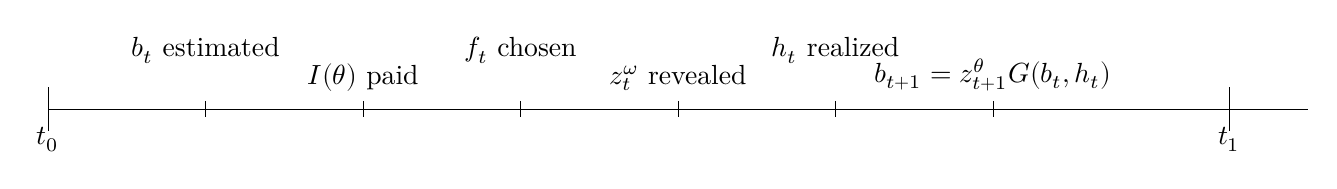
\begin{tikzpicture}
        % draw horizontal line   
        \draw (-8,0) -- (8,0);
    \foreach \x in {-6,-4,-2,0,2,4}
    \draw (\x cm,3pt) -- (\x cm,-3pt);
    \foreach \y in {-8,7}
    \draw (\y cm,8pt) -- (\y cm,-8pt);
    \draw (-8,0) node[below=3pt] {$ t_0 $} node[above=3pt] {$  $};
    \draw (-6,0) node[above=13pt] {$b_t$ estimated};
    \draw (-4,0) node[above=3pt] {$I(\theta)$ paid};
    \draw (-2,0) node[above=13pt] {$f_t$ chosen};
    \draw (0,0) node[above=3pt] {$z_t^\omega$ revealed};
    \draw (2,0) node[above=13pt] {$h_t$ realized};
    \draw (4,0)  node[above=3pt] {$b_{t+1}=z_{t+1}^\theta G(b_t,h_t)$};
    \draw (7,0) node[below=3pt] {$t_1$} ;
\end{tikzpicture}
\caption{Timing of model when insurance contract triggers on $z_t^\omega$} 
    \label{fig:M1}
\end{figure}

An insurance contract built on the harvest shock \(z^\omega_{t+1}\) will
payout at the end of the year after harvest occurs (Figure 2). The
manager will make harvest choices \(f_t\) before knowing whether
insurance will benefit fishers. The effects of a pre or post harvest
payout could be stark. If the manager knows the stock is in poor
condition, they may be more willing to reduce harvest because the
fishers are covered from the closure through the insurance. The stock
could recover faster through the equation of motion. Alternatively, post
harvest payouts may have more subtle influence on how a manager would
define the Harvest Control Rule.

\begin{figure}
    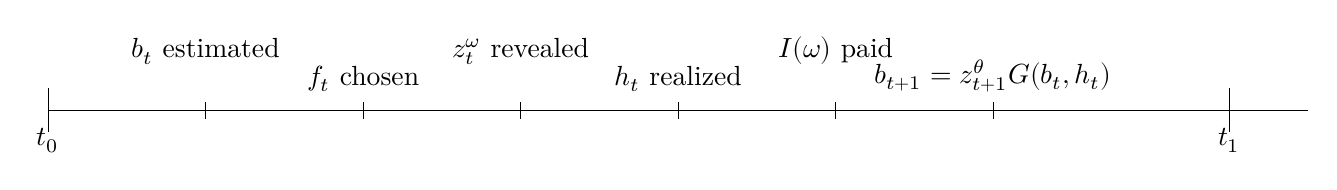
\begin{tikzpicture}
        % draw horizontal line   
        \draw (-8,0) -- (8,0);
    \foreach \x in {-6,-4,-2,0,2,4}
    \draw (\x cm,3pt) -- (\x cm,-3pt);
    \foreach \y in {-8,7}
    \draw (\y cm,8pt) -- (\y cm,-8pt);
    \draw (-8,0) node[below=3pt] {$ t_0 $} node[above=3pt] {$  $};
    \draw (-6,0) node[above=13pt] {$b_t$ estimated};
    \draw (-4,0) node[above=3pt] {$f_t$ chosen};
    \draw (-2,0) node[above=13pt] {$z_t^\omega$ revealed};
    \draw (0,0) node[above=3pt] {$h_t$ realized};
    \draw (2,0) node[above=13pt] {$I(\omega)$ paid};
    \draw (4,0)  node[above=3pt] {$b_{t+1}=z_{t+1}^\theta G(b_t,h_t)$};
    \draw (7,0) node[below=3pt] {$t_1$} ;
\end{tikzpicture}
\caption{Timing of model when insurance contract triggers on $z_t^\omega$} 
\label{fig:M2}
\end{figure}

The Bellman for Equation~\ref{eq-npv} accounts for uncertainty in both
the current and future periods.

\begin{equation}\phantomsection\label{eq-bell}{
\begin{aligned}
V(b_t)=\max_{f_t} \mathbb{E}\left[u(f_t,z_t^\omega,z_t^\theta,I(v))+\beta V(z_{t+1}^\theta G(b_t-h_t))\right]
\end{aligned}
}\end{equation}

The first order conditions that solve Equation~\ref{eq-bell} demonstrate
how insurance and management could complement each other
(Equation~\ref{eq-foc}).

\begin{equation}\phantomsection\label{eq-foc}{
\begin{aligned}
&\mathbb{E}[\pi'(f_t,z_t^\omega)U'(f_t,z_t^\omega,z_t^\theta,I(v))]=\beta \mathbb{E}[G'(b_t-h_t)V'(z_{t+1}^\theta G(b_t-h_t))] \\
&\mathbb{E}[\pi'(f_t,z_t^\omega)]\mathbb{E}[U'(f_t,z_t^\omega,z_t^\theta,I(v))]+\text{cov}[\pi'(f_t,z_t^\omega),U'(f_t,z_t^\omega,z_t^\theta,I(v))] \\
&=\beta \mathbb{E}[G'(b_t-h_t)]\mathbb{E}[V'(z_{t+1}^\theta G(b_t-h_t))] +\text{cov}[G'(b_t-h_t),V'(z_{t+1}^\theta G(b_t-h_t))]
\end{aligned}
}\end{equation}

The expected marginal utility gain from current period harvesting (line
2 of Equation~\ref{eq-foc}) must exactly equal the expected marginal
utility gain of future fish (line 3 of Equation~\ref{eq-foc}). There are
two wealth and investment effects, one for each period. The marginal
value of current profit, \(\mathbb{E}[\pi']\), is the immediate wealth
effect and is matched by future wealth in the marginal value of future
fish stocks \(\mathbb{E}[G'(b_t-h_t)]\).

The investment effect is more nuanced. The risk fishers take on now,
\(\text{cov}[\pi',U']\), has a corresponding risk in the future,
\(\text{cov}[G'(b_t-h_t),V']\), which dictates how much risk fishers are
willing to take on now or later. Insurance will affect both these
effects. Insurance lowers the variance of utility by equalizing bad and
goods states. The covariance of the shocks will lower with less variance
in utility. The relative magnitude of reduction in present or future
covariance will determine how the harvest control rule is defined.
Additionally, it will depend on which wealth effect takes up the margin.
Both of these impacts will depend on the type of insurance contract
specified. For example, a contract built on current period shocks
\(z_t^\omega\) will most likely have a larger impact on the current
period investment effect, lowering \(\text{cov}[\pi',U']\). Does the
manager respond to this reduction by raising immediate harvest to
extract more wealth now\footnote{The structure of the current model is
  implicitly risk increasing in the current period. I would like to
  introduce risk decreasing specifications, but I worry that the
  structural form of risk decreasing harvest will not work in value
  function iteration. The \(f^{-\beta}\) adds huge amounts of risk when
  \(f\) is low. So if the manager needs to close the stock for
  biological purposes, the risk reducing form will never want a closure
  because the risk will be astronomical.} or does the manager lower
harvest in response to the bad state of the world and tradeoff for more
future wealth? The complexity of the problem eliminates tractable
analytical solutions. In the next section I use numerical methods to
approximate the optimal harvest control rule with and without insurance
for a manager with risk averse fisher preferences.

\subsection{Numerical Solution
Methods}\label{numerical-solution-methods}

Dynamic Programming will find the optimal policy function \(f(b^*)\) to
define a harvest control rule for each observed \(b_t\). I consider two
approaches to solve the model, both use Value Function Iteration. The
first approach discretizes the distributions of both shocks into
predefined bins using Markov transition probabilities
(Figure~\ref{fig-omega}). Then the algorithm iterates over each
combination of shocks and states. It maximizes the current expected
utility over each \(z_t^\omega\) and the future utility over each
\(z_t^\theta\) bin by selecting \(f(b^*)\). The algorithm continues to
iterate until the value function \(V(b)\) converges to the same future
value function \(V_{t+1}(b)\).

The first approach suffers from the curse of dimmensionality. More
precise answers require more bins and states. The search space can
become prohibitively large. Approximate dynamic programming uses Monte
Carlo simulation to approximate future value functions after decisions
are made in the current period (Powell 2011). This setting might be
particularly well suited for ADP as I can jointly sample both
\(z_t^\omega\) and \(z_t^\theta\) simultaneously. Expected value of
insurance needs to be calculated through Monte Carlo simulation. The
algorithm will iterate over each \(b_t\) to select \(f(b^*)\) until the
value function converges.

\begin{figure}

\centering{

\pandocbounded{\includegraphics[keepaspectratio]{docs_files/figure-pdf/fig-omega-1.pdf}}

}

\caption{\label{fig-omega}Example of the discretizing the \(z_t^\omega\)
distribution into 13 bins with a log normal distribution and mean 0 and
standard deviation 0.5}

\end{figure}%

\subsection{Structural forms}\label{structural-forms}

I consider two concave utility forms for the fishers: Constant Relative
Risk Aversion and Constant Absolute Risk Aversion. When the risk
aversion parameter \(\eta=1\) I add a sufficient high constant, \(k\) to
profits to ensure I do not take negative logs. This will not interfere
with the optimization procedure as the marginal utility defines the
convergence.

\[
u(\pi,I(v))=\begin{cases}
\frac{\pi^{1-\eta}}{1-\eta} & \text{if } \eta\neq 1 \\
\log(\pi+k) & \text{if } \eta=1
\end{cases}
\]

Convex costs are modeled through a squared cost function. The cost
parameter \(c\) is set to ensure choices of harvest are positive for
most levels of fish stock. Harvest is defined above through
Equation~\ref{eq-harvest}.

\[
\pi(f_t)=p f_t b_tz^\omega_t - c f_t^2
\]

The growth function is a logistic growth function. The growth parameter
\(r\) is set to ensure the stock does not go extinct. Carrying capacity
\(K\) is the upper bound of stock abundance. Next period biomass grows
on the residual escapement of fish after harvest \(s_t=b_t-h_t\).

\[
b_{t+1}=z_{t+1}^\theta \left[s_t+ r s_t(1-\frac{s_t}{K})\right]
\] The multiplicative nature of the shocks require distributions with
\(\mathbb{E}=1\) and all realizations must be greater than 0. Lognormal
distributions provide both properties by ammending the \(mu\) parameter
of the distribution. Lognormal distributions in expectation are
\(\mathbb{E}[X]=\exp(\mu+\frac{1}{2}\sigma^2)\). Setting the expectation
to 1 and solving for \(mu\) in terms of \(\sigma^2\) allows me to center
the distribution around 1 with only positive shocks.

\[
\begin{aligned}
z_t^\omega &\sim \text{Lognormal}(-\frac{1}{2}\sigma^2_\omega,\sigma^2_\omega) \\
z_t^\theta &\sim \text{Lognormal}(-\frac{1}{2}\sigma^2_\theta,\sigma^2_\theta)
\end{aligned}
\]

\section{Preliminary Results}\label{sec-res}

I test a quick preliminary run of the model using only the growth shock
and the Markov transition probability approach. Index insurance appears
to reduce the optimal HCR at all levels of biomass
(Figure~\ref{fig-hcr}). The new policy function slightly approaches a
risk neutral specification. This matches predictions that insurance
allows risk averse users to behave more like risk neutral ones.

\begin{figure}

\centering{

\pandocbounded{\includegraphics[keepaspectratio]{docs_files/figure-pdf/fig-hcr-1.pdf}}

}

\caption{\label{fig-hcr}Optimal harvest control rules with insurance
(yellow), no insurance (blue), and a risk neutral manager (green) with
no insurance.}

\end{figure}%

At all levels of biomass, insurance reduces harvest relative to the risk
averse manager with no insurance (Figure~\ref{fig-pct}). The overall
effect is small, but the percent difference in harvest can be quite
large especially at low levels of biomass. Managers are more inclined to
invest in future wealth of the stock if uncertainty in the current
period is reduced. Insurance allows managers to purse strategies that
reduce harvest pressure on the stock, increasing future value and
providing biological conservation.

\begin{figure}

\centering{

\pandocbounded{\includegraphics[keepaspectratio]{docs_files/figure-pdf/fig-pct-1.pdf}}

}

\caption{\label{fig-pct}Percent difference in optimal harvest control
rules between insurance and no insurance at every level of biomass.}

\end{figure}%

\section{Future Steps}\label{sec-fut}

The results of the preliminary analysis are promising, but there remain
several steps to complete. The necessary goals are summarized below with
strategies to resolve each.

\begin{itemize}
\tightlist
\item
  \textbf{Expand to two shock framework}
\end{itemize}

The model currently only considers the growth shock.

\begin{itemize}
\tightlist
\item
  \textbf{Introduce basis risk}
\end{itemize}

Allowing the shocks to be correlated with each other can act as a proxy
for basis risk. Basis risk is detrimental to the uptake of insurance.
Assuming independence implies there will always be a residual amount of
risk that cannot be insured. The degree to which the shocks are
correlated could impact the structure of the HCR in unexpected ways.

A copula will link the weather variables together for correlation
coefficients between 0 and 1. Copulas are preferred in this instant as
they allow me to easily specify an correlation and distribution for both
shocks. The VFI solutions will sample from the multivariate copula to
extract harvest and biological shocks. The VFI procedure will be
repeated for each to assess the impact of basis risk on the HCR.

\begin{itemize}
\tightlist
\item
  \textbf{Model Robustness Checks}
\end{itemize}

There are a variety of parameters that need to be checked to understand
the full range of impacts insurance will have on the HCR. The amount of
insurance \(\gamma\) for either contract needs to be varied to ensure
that optimal insurance coverage is selected to not bias the results with
over or under insurance. The smoothness of the Value function will
determine whether \(\gamma\) could be included as a choice variable in
Equation~\ref{eq-bell}. The jaggedness of the converged value function
in Figure~\ref{fig-hcr} indicates this may be problematic. Instead, I
will vary \(\gamma\) from 0 to pre-insurance profits at Maximum
Sustainable Yield levels of biomass to identify an optimal value of
\(\gamma\).

Risk aversion and the time value of utility will also affect the impacts
of insurance on the optimal HCR policy. Greater risk aversion may lead
to increased insurance value that encourages stronger responses from the
manager. The isoelastic parameter \(\eta\) will be varied with
reasonable estimates from the financial literature or possibly from
studies that calculate fisher risk aversion. The discount rate will also
be varied to adjust the time value of money.

Lastly, the relative and absolute amounts of variance from the shocks
will be tested assess the changes in the optimal HCR. Sethi \emph{et
al.} (2005) showed more variance from measurement error shock that is
similar to my \(z_t^\omega\) has large impacts on the optimal HCR.
Insurance mitigates these risks and the amount of correlation between
this shows could provide interesting interactions as a result.

\begin{itemize}
\tightlist
\item
  \textbf{Simulate the stock and fisher benefits with new policy
  function}
\end{itemize}

The model will be simulated with the new policy function to assess the
impacts of insurance on the stock and fisher income. Probability of
stock extinction after 50 years will be calculated for each optimal
insurance policy\footnote{In the event that the HCR do not lead to
  extinction, I will calculate the mean and variance of stock levels at
  50 years}. Monte Carlo simulation with 1,000 draws of 50 years will
use the HCR and growth function to examine the distribution of stock
health and fisher utility.

\newpage{}

\textbf{Using Mahul and Ramaswami style proof}

Each term can be decomponsed by the definition of covariance:

\[
\begin{aligned}
\partial u_n&=\mathbb{E}[\frac{\partial u(\pi(f_1,b_1,w_1),I(w))]}{\partial f_1} \mathbb{E}[\frac{\partial \pi(f_1,b_1,w_1)}{\partial f_1}]+\text{cov}(\frac{\partial u}{\partial f_1},\frac{\partial \pi(b_1,f_1,w)}{\partial f_1}) \\
\partial u_f&=\beta\left(\mathbb{E}[\frac{\partial u(\pi(G(s),f_2,w_2),I(w_1))}{\partial f_1}] \mathbb{E}[\frac{\partial \pi(G(s),f_2,w_2)}{\partial f_1}]+\text{cov}(\frac{\partial u}{\partial f_1},\frac{\partial \pi(G(s),f_2,w_2)}{\partial f_1})\right)
\end{aligned}
\]

For a risk averse fishers,
\(0>cov(\partial u(f_1,b_1,I(w))/\partial f_1,\partial \pi(b_1,f_1,w)/\partial f_1)>cov(\partial u(f_1,b_1,0)/\partial f_1,\partial \pi(b_1,f_1,)/\partial f_1)\)
if \(\partial V(\pi(f_1,b_1,w)/ \partial f_1>0\).
\(0<cov(\partial u(f_1,b_1,I(w)/\partial f_1,\partial \pi(b_1,f_1,w)/\partial f_1)<cov(\partial u(f_1,b_1,0)/\partial f_1,\partial \pi(b_1,f_1,)/\partial f_1)\)
if \(\partial V(\pi(f_1,b_1,w)/ \partial f_1>0\). :::\{\#prp-twocur\}

The proof of \#prp-twocur is included in the appendix. The outcome of
\#prp-twocur is that insurance has two incentive pathways to adjust
current period harvest. First, current period utility \(\partial u_n\)
uses a risk increasing input. Insurance alleviates this constraint
incentivizing additional harvest as shown in (\textbf{Grimes2025?}),
Mahul (2001), and Ramaswami (1993).

Current period harvest is a risk decreasing input in the future period.
Therefore, insurance will lower harvest in the current period. Current
period harvest acts as a risk decreasing input because it lowers the
amount of biomass in the next period. Biomass captures the randomness of
the second period. Fewer fish in the next period implicitly lowers the
variance of the next period. Insurance will protect against future
flucutations so that fishers are incentivized to decrease harvest now.

It is impossible to sign the overall effect of insurance as it is the
additive combination of the marginal changes in \(\partial u_n\) and
\(\partial u_f\). However, the discount rate will probably skew the
change towards more short term harvest as future harvest is less
valuable. The magnitude of difference may also be dependent on the
initial level of biomass \(b_1\) because the growth rate depends on the
standing stock available.

\section*{References}\label{references}
\addcontentsline{toc}{section}{References}

\phantomsection\label{refs}
\begin{CSLReferences}{1}{0}
\bibitem[\citeproctext]{ref-Andersen1984}
Andersen, P. and Sutinen, J.G. (1984) Stochastic bioeconomics: A review
of basic methods and results.

\bibitem[\citeproctext]{ref-Bellido2020}
Bellido, J.M., Sumaila, U.R., Sánchez-Lizaso, J.L., Palomares, M.L. and
Pauly, D. (2020)
\href{https://doi.org/10.1016/J.MARPOL.2019.103786}{Input versus output
controls as instruments for fisheries management with a focus on
mediterranean fisheries}. \emph{Marine Policy} \textbf{118}.

\bibitem[\citeproctext]{ref-Bellquist2021}
Bellquist, L., Saccomanno, V., Semmens, B.X., Gleason, M. and Wilson, J.
(2021) \href{https://doi.org/10.7717/peerj.11186}{The rise in climate
change-induced federal fishery disasters in the united states}.
\emph{PeerJ} \textbf{9}.

\bibitem[\citeproctext]{ref-Bradley2019}
Bradley, D., Merrifield, M., Miller, K.M., Lomonico, S., Wilson, J.R.
and Gleason, M.G. (2019)
\href{https://doi.org/10.1111/faf.12361}{Opportunities to improve
fisheries management through innovative technology and advanced data
systems}. \emph{Fish and Fisheries} \textbf{20}, 564--583.

\bibitem[\citeproctext]{ref-Bulte2021}
Bulte, E. and Haagsma, R. (2021)
\href{https://doi.org/10.1007/s10640-021-00545-1}{The welfare effects of
index-based livestock insurance: Livestock herding on communal lands}.
\emph{Environmental and Resource Economics} \textbf{78}, 587--613.

\bibitem[\citeproctext]{ref-Cheung2018}
Cheung, W.W.L., Jones, M.C., Reygondeau, G. and Frölicher, T.L. (2018)
\href{https://doi.org/10.1111/gcb.14390}{Opportunities for climate-risk
reduction through effective fisheries management}. \emph{Global Change
Biology} \textbf{24}, 5149--5163.

\bibitem[\citeproctext]{ref-Clark1986}
Clark, C.W. and Kirkwood, G.P. (1986) On uncertain renewable resource
stocks: Optimal harvest policies and the value of stock surveys*.

\bibitem[\citeproctext]{ref-Costello2012}
Costello, C., Ovando, D., Hilborn, R., Gaines, S.D., Deschenes, O. and
Lester, S.E. (2012)
\href{https://doi.org/10.1126/science.1227123}{Status and solutions for
the world's unassessed fisheries}. \emph{Science} \textbf{338},
514--517.

\bibitem[\citeproctext]{ref-Dichmont2010}
Dichmont, C.M., Pascoe, S., Kompas, T., Punt, A.E. and Deng, R. (2010)
\href{https://doi.org/10.1073/pnas.0912091107}{On implementing maximum
economic yield in commercial fisheries}. \emph{Proceedings of the
National Academy of Sciences of the United States of America}
\textbf{107}, 16--21.

\bibitem[\citeproctext]{ref-Free2023}
Free, C.M., Mangin, T., Wiedenmann, J., Smith, C., McVeigh, H. and
Gaines, S.D. (2023) \href{https://doi.org/10.1111/faf.12724}{Harvest
control rules used in US federal fisheries management and implications
for climate resilience}. \emph{Fish and Fisheries} \textbf{24},
248--262.

\bibitem[\citeproctext]{ref-Grainger2013}
Grainger, C.A. and Parker, D.P. (2013)
\href{https://doi.org/10.1146/annurev-resource-091912-151838}{The
political economy of fishery reform}. \emph{Annual Review of Resource
Economics} \textbf{5}, 369--386.

\bibitem[\citeproctext]{ref-Hilborn2020}
Hilborn, R., Amoroso, R.O., Anderson, C.M., et al. (2020)
\href{https://doi.org/10.1073/pnas.1909726116/-/DCSupplemental}{Effective
fisheries management instrumental in improving fish stock status}.
\emph{PNAS} \textbf{117}, 2218--2224.

\bibitem[\citeproctext]{ref-Hilborn2014}
Hilborn, R. and Ovando, D. (2014)
\href{https://doi.org/10.1093/icesjms/fsu034}{Reflections on the success
of traditional fisheries management}. \emph{ICES Journal of Marine
Science} \textbf{71}, 1040--1046.

\bibitem[\citeproctext]{ref-Hoefnagel2017}
Hoefnagel, E. and Vos, B. de (2017)
\href{https://doi.org/10.1016/j.marpol.2016.09.019}{Social and economic
consequences of 40 years of dutch quota management}. \emph{Marine
Policy} \textbf{80}, 81--87.

\bibitem[\citeproctext]{ref-Jardine2020}
Jardine, S.L., Fisher, M.C., Moore, S.K. and Samhouri, J.F. (2020)
\href{https://doi.org/10.1016/j.ecolecon.2020.106691}{Inequality in the
economic impacts from climate shocks in fisheries: The case of harmful
algal blooms}. \emph{Ecological Economics} \textbf{176}.

\bibitem[\citeproctext]{ref-Percy2020}
Jeremy, B.P. and O'Riordan (2020)
\href{https://doi.org/10.1007/978-3-030-37371-9_2}{The EU common
fisheries policy and small-scale fisheries: A forgotten fleet fighting
for recognition}. In: \emph{Small-Scale Fisheries in Europe: Status,
Resilience and Governance}. (eds Cristina, B.M.P.-F.J. J. and Pita).
Springer International Publishing, pp 23--46.

\bibitem[\citeproctext]{ref-Kelsall2023}
Kelsall, C., Quaas, M.F. and Quérou, N. (2023)
\href{https://doi.org/10.1016/j.jeem.2023.102855}{Risk aversion in
renewable resource harvesting}. \emph{Journal of Environmental Economics
and Management} \textbf{121}.

\bibitem[\citeproctext]{ref-Kvamsdal2016}
Kvamsdal, S.F., Eide, A., Ekerhovd, N.A., et al. (2016)
\href{https://doi.org/10.12952/journal.elementa.000114}{Harvest control
rules in modern fisheries managementharvest control rules in modern
fisheries management}. \emph{Elementa} \textbf{2016}.

\bibitem[\citeproctext]{ref-Lane1998}
Lane, D.E., Lane, R.L.S. and Stephenson, D.E. (1998) A framework for
risk analysis in fisheries decision-making. \emph{ICES Journal of Marine
Science} \textbf{55}, 1--13.

\bibitem[\citeproctext]{ref-Lewis1981}
Lewis, T.R. (1981) Exploitation of a renewable resource under
uncertainty. \textbf{14}, 422--439.

\bibitem[\citeproctext]{ref-Liu2016}
Liu, O.R., Thomas, L.R., Clemence, M., Fujita, R., Kritzer, J.P.,
McDonald, G. and Szuwalski, C. (2016)
\href{https://doi.org/10.1080/23308249.2016.1161002}{An evaluation of
harvest control methods for fishery management}. \emph{Reviews in
Fisheries Science and Aquaculture} \textbf{24}, 244--263.

\bibitem[\citeproctext]{ref-Ludwig1979}
Ludwig, D. (1979) \href{https://epubs.siam.org/terms-privacy}{OPTIMAL
HARVESTING OF a RANDOMLY FLUCTUATING RESOURCE. I: APPLICATION OF
PERTURBATION METHODS*}. \emph{SIAM J. APPL. MATH} \textbf{37}.

\bibitem[\citeproctext]{ref-Mahul2001}
Mahul, O. (2001) \href{https://doi.org/10.1111/0002-9092.00180}{Optimal
insurance against climatic experience}. \emph{American Journal of
Agricultural Economics} \textbf{83}, 593--604.

\bibitem[\citeproctext]{ref-Mangin2018}
Mangin, T., Costello, C., Anderson, J., et al. (2018)
\href{https://doi.org/10.1371/journal.pone.0204258}{Are fishery
management upgrades worth the cost?} \emph{PLoS ONE} \textbf{13}.

\bibitem[\citeproctext]{ref-muller2011}
Müller, B., Quaas, M.F., Frank, K. and Baumgärtner, S. (2011)
\href{https://doi.org/10.1016/j.ecolecon.2011.06.011}{Pitfalls and
potential of institutional change: Rain-index insurance and the
sustainability of rangeland management}. \emph{Ecological Economics}
\textbf{70}, 2137--2144.

\bibitem[\citeproctext]{ref-Pares2015}
Parés, C., Dresdner, J. and Salgado, H. (2015)
\href{https://doi.org/10.1016/j.marpol.2014.12.011}{Who should set the
total allowable catch? Social preferences and legitimacy in fisheries
management institutions}. \emph{Marine Policy} \textbf{54}, 36--43.

\bibitem[\citeproctext]{ref-Powell2011}
Powell, W.B. (2011) \emph{Approximate dynamic programming: Solving the
curses of dimensionality}, 2nd edn. John Wiley \& Sons.

\bibitem[\citeproctext]{ref-Punt2010}
Punt, A.E. (2010) Harvest control rules and fisheries management. In:
\emph{Handbook of Marine Fisheries Conservation and Management}. (eds
R.Q. Grafton, R. Hilborn, D. Squire, M. Tait and M.J. Williams). Oxford
University Press, pp 582--594.

\bibitem[\citeproctext]{ref-Ramaswami1993}
Ramaswami, B. (1993) Supply response to agricultural insurance: Risk
reduction and moral hazard effects. \emph{American Journal of
Agricultural Economics} \textbf{75}, 914--925.

\bibitem[\citeproctext]{ref-Reed1979}
Reed, W.J. (1979) Optimal escapement levels in stochastic and
deterministic harvesting models *. \emph{Journal of Environmental
Economics and Management}, 350--363.

\bibitem[\citeproctext]{ref-Santora2020}
Santora, J.A., Mantua, N.J., Schroeder, I.D., et al. (2020)
\href{https://doi.org/10.1038/s41467-019-14215-w}{Habitat compression
and ecosystem shifts as potential links between marine heatwave and
record whale entanglements}. \emph{Nature Communications} \textbf{11}.

\bibitem[\citeproctext]{ref-Sethi2005}
Sethi, G., Costello, C., Fisher, A., Hanemann, M. and Karp, L. (2005)
\href{https://doi.org/10.1016/J.JEEM.2004.11.005}{Fishery management
under multiple uncertainty}. \emph{Journal of Environmental Economics
and Management} \textbf{50}, 300--318.

\bibitem[\citeproctext]{ref-Sethi2010}
Sethi, S.A. (2010)
\href{https://doi.org/10.1111/j.1467-2979.2010.00363.x}{Risk management
for fisheries}. \emph{Fish and Fisheries} \textbf{11}, 341--365.

\bibitem[\citeproctext]{ref-Szuwalski2023}
Szuwalski, C.S., Aydin, K., Fedewa, E.J., Garber-Yonts, B. and Litzow,
M.A. (2023) \href{https://doi.org/10.1126/SCIENCE.ADF6035}{The collapse
of eastern bering sea snow crab}. \emph{Science} \textbf{382}, 306--310.

\bibitem[\citeproctext]{ref-Watson2023}
Watson, J.R., Spillman, C.M., Little, L.R., Hobday, A.J. and Levin, P.S.
(2023) \href{https://doi.org/10.1093/icesjms/fsad175}{Enhancing the
resilience of blue foods to climate shocks using insurance}. \emph{ICES
Journal of Marine Science} \textbf{80}, 2457--2469.

\bibitem[\citeproctext]{ref-Yamazaki2009}
Yamazaki, S., Kompas, T. and Grafton, R.Q. (2009)
\href{https://doi.org/10.1111/j.1939-7445.2008.00034.x}{Output versus
input controls under uncertainty: The case of a fishery}. \emph{Natural
Resource Modeling} \textbf{22}, 212--236.

\end{CSLReferences}




\end{document}
